%%%%%%%%%%%%%%%%%%%%%%%%%%%%%%%%%%%%%%
% START ADDING TEXT HERE
%
% Feel free to use \include commands to structure text in smaller
% pieces
%
%%%%%%%%%%%%%%%%%%%%%%%%%%%%%%%%%%%%%%


% Abstract gives a brief summary of the main points of a paper:
\begin{abstract}
\textbf{Abstract - }
\end{abstract}

% the actual content, usually separated over a number of sections
% each section is assigned a label, in order to be able to put a
% crossreference to it

\section{Introduction}
\label{sec:introduction}
In recent years with the evolution of technology, Internet of Things (IoT) devices are increasing day by day. According to Ericsson mobility report\cite{}, there will be 17\% (approx. 22.3 billion) increase in IoT devices by 2024. Functionally IoT is defined as \emph{"The Internet of Things allows people and things to be connected Anytime, Anyplace, with Anything and Anyone"} \cite{European commission 2008}. IoT devices have served mankind in many ways such as from smart houses to smart cities, smart transportation systems and many medical applications. These IoT applications enables many devices connected to network and generates alot of heterogeneous data also known as BigData which requires special data processing models and Infrastructure support. Processing BigData required alot of resources and cloud computing theoratically provides it unlimited resources\cite{fog-comp-survey}. But there is downside of using cloud computing for such complex computation as it is more costly when it comes to computation power, storage and bandwidth. Computation need to be performed at the node level and only the aggregated data need to send to central node for further computations and analysis. This de-centralized approach will save alot of computation power as well as bandwidth requriments\cite{fog-comp-survey}. To overcome the downside of cloud computing, the terminology fog computing is used. Fog computing allows the computation at the egde of network instead of central core. \par
Fog computing is defined as \emph{"an archietecture that uses one or a collaborative multitude of end-user clients or near-user edge devices to carry out a substantial amount of storage (rather than stored primarily in cloud data centers), communication (rather than routed over the internet backbone), and control, configuration, measurement and management (rather than controlled primarily by network gateways such as those in the LTE (telecommunication) core)”}\cite{Chiang 2015; Aazam and Huh 2014}. Traditionally, user applications running in cloud access the cloud core network through access points for data exchange to fetch data from data-centers \cite{Bittencourt2017}. In fog computing these access points also serves as resource providers such as computation power and storage etc. and are called "cloudlets"\cite{Bittencourt2017}. Figure \ref{fig:fog-arch} show the top-level archietecture of the fog computing. \par
\begin{figure}
  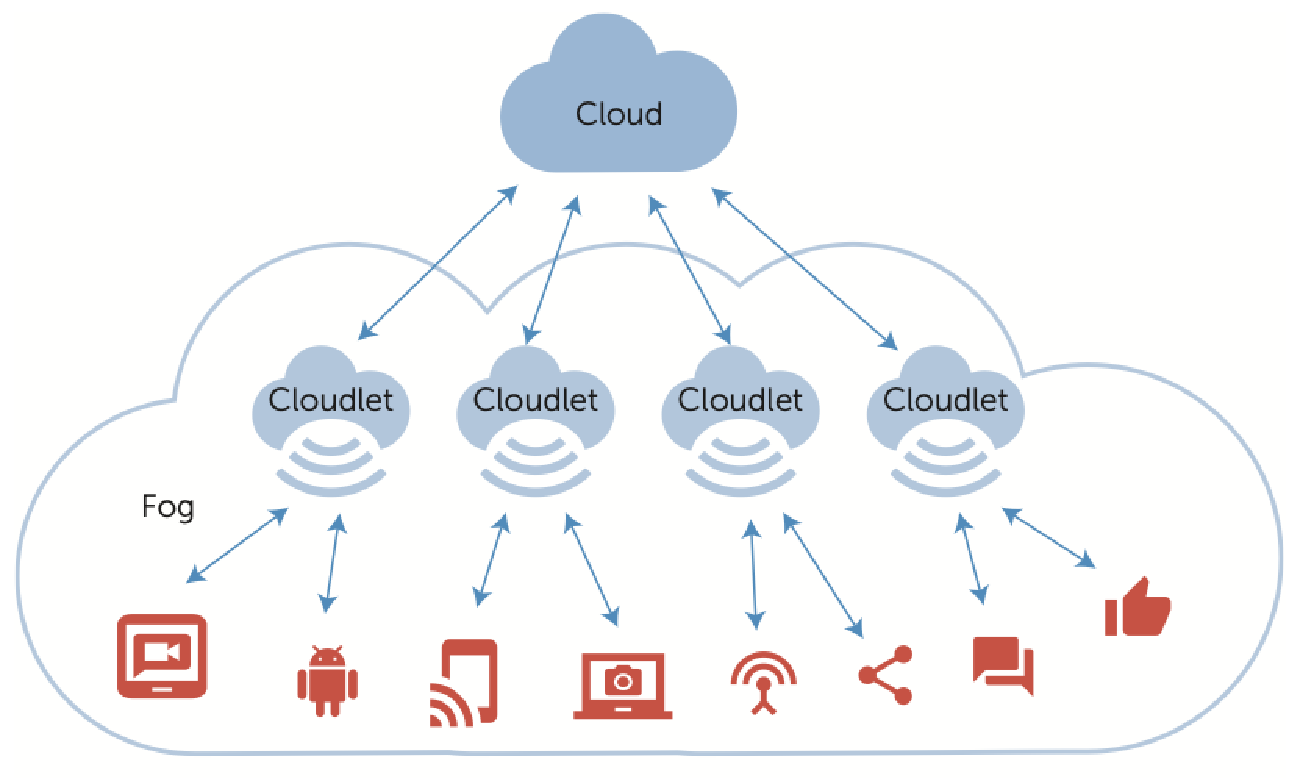
\includegraphics[width=70mm]{figures/mlcn-fog-1.pdf}
  \caption{Fog computing: Top-level overview\cite{Bittencourt2017}}
  \label{fig:fog-arch}
\end{figure}
Fog computing is responsible for providing resources to IoT devices for processing. Traditionally these resources are allocated as VMs from different cloud infrastructures such as AWS, Google, OpenStack, etc. to run the applications. VMs are considered resource greedy and require more computational resources. Alternate is to use the Containers such as Docker which are light-weight, requires less resources and based on micro-service architecture. Large applications are split into containers based on the main processes of the application. This increasing number of containers per application required the proper monitoring for health check and resource consumption. The most commonly used orchestrator for containers is Kubernetes. \par
Kubernetes act as IaaS for fog computing to provide resource for IoT applications. Kubernetes is an open-source platform for management, deployment and scaling of containers. In Kubernetes, applications are deployed as pod consisting of multiple containers. When the configuration of deploying application is passed to Kubernetes, it checks for the availability of resources and deploys afterward. Kubernetes default resource scheduler monitor and deploys the pod using computation power-based scheduling mechanism and does not consider latency and available bandwidth, which is considered important while dealing with data-centric application. Example of data-centric application is weather forecast that receives data from scattered IoT devices and provide prediction. If the data is lost or delayed due higher latency and poor bandwidth, timely decisions cannot be made that leads to disaster. To overcome this drawback of Kubernetes, author proposed an alternate Kubernetes scheduler that consider network resources along with computational resources.
\section{Backgroud}
\label{sec:backgroud}
\begin{itemize}
  \item Kubernetes Internal Archietecture and Main Components
  \item Kubernetes works as an Orchestrator
  \item Kubernetes resource provisioning
  \item Concluding the section with pitfals of default scheduler of Kubernetes
\end{itemize}
This section explains about the Kubernetes main components, working as Orchestrator and built-in resource provisioning techniques.
\subsection{Kubernetes Main Components}
\label{sec:k8s_main_comp}
\begin{figure}
  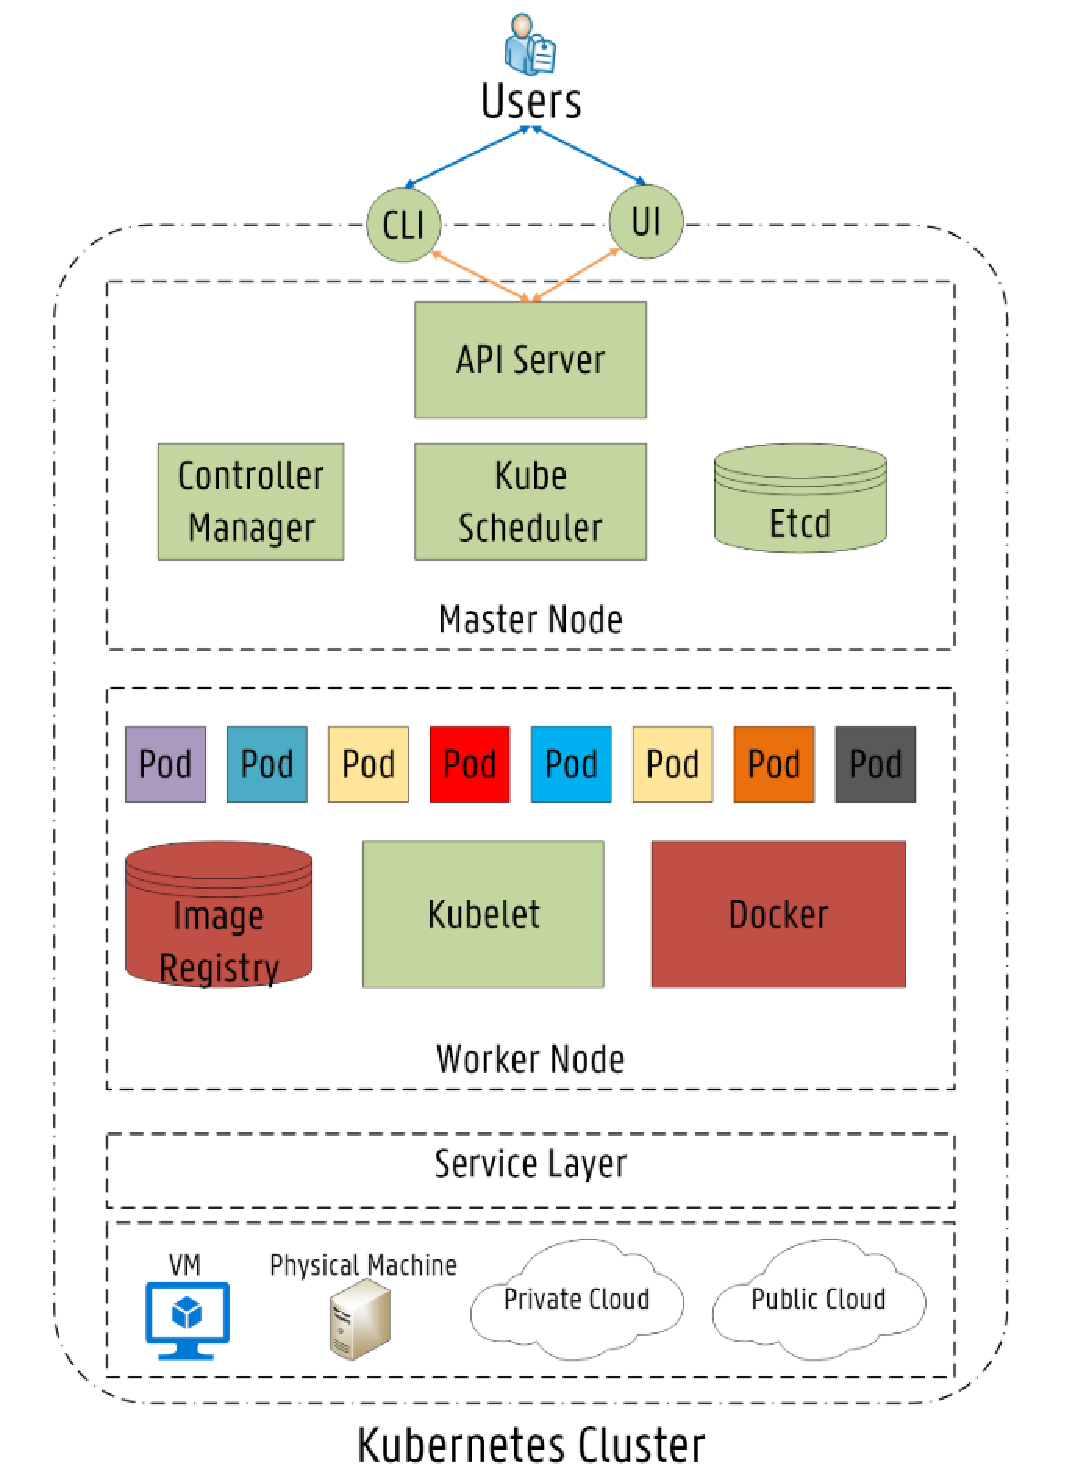
\includegraphics[width=70mm]{figures/mlcn-k8s-components.pdf}
  \caption{Kubernetes Cluster: Main Components\cite{Santos2019}}
  \label{fig:k8s-comp}
\end{figure}
Kubernetes is an open-source project that manages the container-based applications deployed over multiple hosts. Kubernetes act as Orchestrator which is responsible for deploying, managing, scaling of container-based application\cite{kubernetes-github-repo}. Figure \ref{fig:k8s-comp} shows the main components coupled to work as one unit called kubernetes. It is based on master-slave model, consisting of one \emph{master node} and multiple \emph{worker nodes} \cite{Santos2019}. \emph{worker nodes} can be either physical or virtual resource such as physical servers or virtual machines. \emph{master node} communicates with \emph{worker nodes} using \emph{API} calls. \emph{API server} uses RESTFul API, for managing all the \emph{API} calls is also part of \emph{master node}. End-users communicates with kubernetes cluster using \emph{Kubectl}, which forward user requests to \emph{API server} and intern gets the result. \emph{Etcd} stores the data as key-value pair,which is used to store all configurations, states. It is one of the main component of kubernetes, which maintians the state across the cluster for synchorization of data. \emph{Control Manager} is resposible for monitoring of \emph{Etcd}. For any state change of cluster, \emph{Control Manager} forward the new state request using \emph{API server}. \emph{Kube Scheduler} is later in section \ref{sec:k8s_scheduler}. On \emph{worker node}, node agent known as \emph{Kubelet} which is resposible for maintain state based on \emph{API server} request. For any state change communicated by \emph{API server}, \emph{Kubelet} performs the desired operation such as starting or deleting of Docker containers. \emph{Image Registry} is resposible for managing the images required to create the container applications. \emph{Pod} is main component of \emph{worker node} where all the applications are deployed. Single \emph{Pod} represents the application which consists of multiple containers based on the services of application. \emph{Pod} is the collections of containers, volumes in an isolated environment which means there is no cross communication between two \emph{Pods}. Containers running in a \emph{Pod} share the same IP Address \cite{Santos2019}. Containers communicates using different ports, hence there is a limitaion to this apporach as two containers listening on same port cannot be in same \emph{Pod}\cite{Santos2019}.
\subsection{Kubernetes as Orchestrator}
\label{sec:k8s_orchestrator}
\begin{itemize}
  \item Orchestrator main functions
  \item Comparison of available Orchestrator (OpenStack vs Kubernetes)
  \item Workflow of Kubernetes as an Orchestrator (steps)
\end{itemize}

\subsection{Kubernetes Resource Provisioning}
\label{sec:k8s_scheduler}
\begin{itemize}
  \item write about the default Kubernetes scheduler
  \item its main Components
  \item workflow of default scheduler
\end{itemize}

\section{Kubernetes Network-based Resource Provisioning}
\label{sec: k8s_ns}
\begin{itemize}
  \item write about why we need network-based resource provisioning
  \item main factors consideration (e.g bandwidth and latency)
  \item workflow of network-based scheduler
\end{itemize}

\section{Performance Evaluation}
\label{sec:Performance_eval}
\begin{itemize}
  \item Write about the considered use-case of Fog Computing for Evaluation
\end{itemize}
\subsection{Expermentation Setup}
\label{sec:setup}
\begin{itemize}
  \item setup of Kubernetes base on the mentioned use-case of Fog Computing with diagram
\end{itemize}

\subsection{Analysis of Kubernetes Default and Network-based Resource Provisioning}
\label{sec:analysis}
\begin{itemize}
  \item write about the Performance difference between default Kubernetes scheduler and network based scheduler with supporting result tables and graphs
\end{itemize}

\section{Comparison of Network-based Resource Provisioning Solutions}
\label{sec:related_work}
\begin{itemize}
  \item Compare different solutions based on the following criteria:
\end{itemize}

\subsection{Orchestrator}
\label{sec:infra}
\begin{itemize}
  \item write about the differences between Kubernetes(main-paper)\cite{Santos2019} and other available cloud solutions such as Fogernetes\cite{Wobker2018} and \cite{Reale}.
\end{itemize}

\subsection{Resource Provisioning Techniques}
\begin{itemize}
  \item difference between different resource scheduling techniques such  as \cite{Bittencourt2017}, \cite{Haja2019} etc.
\end{itemize}

\section{Conclusion}
\label{sec:concl}

\section{Further Research Topics}
\label{sec:research}
\begin{itemize}
  \item after writing the seminar, if there is any improvement that can be done, will be added in this section.
\end{itemize}
